% vim: set filetype=tex spell:

%Background Chapter : Recount the work that crank did

\chapter{Background}

\label{ch:BG}

%NOTE: this wording is similar to Crank 1.6

The \ac{LPMT} was originally designed in 1971 by Dr. Michael Polites. It was refined into a stabilization system by Dr. Donald Mentch for his masters degree in 2003 and further refined into a system for the \ac{ARC} as his doctoral work \cite{Mentch11}.

\section{\aclp{LPMT}}

The \ac{ARC} \ac{ACDS} uses \acfp{LPMT} to produce the torque needed to properly orient the CubeSat. The torque of the \acp{LPMT} is generated by crossing the dipole moment of the torquer with the local magnetic field as shown in \autoref{eqn:magtorque} where $\vec{m}$ is the magnetic dipole moment of the torquer and $\vec{B}$ is the local magnetic field.
\begin{equation}
\vec{\tau} = \vec{m} \cross \vec{B}
\label{eqn:magtorque}
\end{equation}
This is the same way that torque rods and torque coils have been used on other CubeSats \todo{look for reference}. The unique part about \acp{LPMT} is that the magnetic dipole moment comes from the core of the torquer and does not depend on a continuous current flow to create torque.


\subsection{Hard Magnetic Core}

The cores of the \acp{LPMT} are made of a hard magnetic material that ideally have a saturation curve that looks like \autoref{fig:histlpmt}. The \ac{LPMT} operates by switching the cores between the saturation points, $M_s$ and $-M_s$. The \ac{LPMT} cores are driven to saturation using a capacitor to provide a current pulse through a solenoid. Even after current stops flowing through the solenoid the core will have a dipole moment of $\pm M_r$ depending on which direction the current was run in \cite{Mentch11}.

\begin{figure}[H]
    \centering
    \begin{tikzpicture}

    \def\Ms{2.0}
    \def\Hs{1.8}
    %draw axis
    \draw[<->] (-\Hs-0.5,0) -- (\Hs+0.5,0);
    \draw[<->] (0,-\Ms-0.5) -- (0,\Ms+0.5);

    %black lines that point back to the origin
    \draw[->] (\Hs,\Ms) -- (\Hs,0);
    \draw[->] (-\Hs,-\Ms) -- (-\Hs,0);
    
    %draw axis lables
    \draw (0,\Ms+0.25) node[anchor=east] {$M$};
    \draw (\Hs+0.25,0) node[anchor=north] {$H$};

    %green lines, magnetization in one direction
    \draw[->,green,very thick] (0,\Ms) -- (-0.2,\Ms);
    \draw[->,green,very thick] (-0.2,\Ms) -- (-\Hs,-\Ms);
    \draw[->,green,very thick] (-\Hs-0.7,-\Ms) -- (0,-\Ms);

    %yellow lines, magnetization in the other direction
    \draw[->,blue,very thick] (0,-\Ms) -- (0.2,-\Ms);
    \draw[->,blue,very thick] (0.2,-\Ms) -- (\Hs,\Ms);
    \draw[->,blue,very thick] (\Hs +0.7,\Ms) -- (0,\Ms);

    %draw lables
    \draw (-\Hs,-\Ms) node[anchor=north] {$-M_s$};
    \draw (\Hs,\Ms) node[anchor=south] {$M_s$};

    \draw (-\Hs,0) node[anchor=north east] {$-H_s$};
    \draw (\Hs,0) node[anchor=south west] {$H_s$};

    \draw (0,-\Ms) node[anchor=south east] {$-M_r$};
    \draw (0,\Ms) node[anchor=north west] {$M_r$};


    \end{tikzpicture}
    \caption{Idealized core material hysteresis loop  }
    \label{fig:histlpmt}
\end{figure}

\subsection{Torquer Pair}

%TODO: add discussion of position (in)dependence of torquer par torque

The cores of the \acp{LPMT} are driven to saturation in the direction of the rod. This gives two possible states for each rod. Because in both states the rod generates a net dipole moment the rods are operated in pars so that three possible dipole moments can be produced as shown in \autoref{fig:moments}, where M is the dipole moment of a single torquer.

\begin{figure}[H]
    \centering
    \begin{tikzpicture}
    \def\L{1.5}     %define arrow length
    \draw[->,red,very thick] (1  , 0) -- (1  ,\L);
    \draw[->,red,very thick] (1.5, 0) -- (1.5,\L);
    \draw (1.25,-0.5) node {+2M};

    \draw[->,red,very thick] (3  ,\L) -- (3  , 0);
    \draw[->,red,very thick] (3.5, 0) -- (3.5,\L);
    \draw (3.25,-0.5) node {0M};

    \draw[->,red,very thick] (5  ,\L) -- (5  , 0);
    \draw[->,red,very thick] (5.5,\L) -- (5.5, 0);
    \draw (5.25,-0.5) node {-2M};
    \end{tikzpicture}
    \caption{Possible dipole moments for a torquer pair}
    \label{fig:moments}
\end{figure}

Because each \ac{LPMT} pair can only produce three distinct values of dipole moment, the output of a \ac{LPMT} algorithm must be quantized.

\begin{figure}[H]
    \centering
    \begin{tikzpicture}

    \draw[<->,green,very thick] (2,2) -- (1,2) -- (1,0) -- (-1,0) -- (-1,-2) -- (-2,-2);

    %draw axis
    \draw[<->] (-3,0) -- (3,0);
    \draw[<->] (0,-3) -- (0,3);

    %draw axis labels
    \draw (0,3) node[anchor=south] {$m_{command_q}$};
    \draw (3,0) node[anchor=west] {$m_{command}$};

    \draw (2,0)  node[anchor=north] {$+2M$};
    \draw (1,0)  node[anchor=north] {$+1M$};
    \draw (-1,0) node[anchor=south] {$-1M$};
    \draw (-2,0) node[anchor=south] {$-2M$};

    \draw (0,2)  node[anchor=east] {$+2M$};
    \draw (0,-2) node[anchor=west] {$-2M$};

    \end{tikzpicture}
    %\caption{Quantization function for \acs{LPMT}\protect\cite{Mentch11}}
    \caption{Quantization function for \acs{LPMT}}
    \todo[inline]{Figure reproduced from Crank}
    \label{fig:lpmtq}
\end{figure}

\section{Detumble Algorithm (Mode 1)}

The purpose of the detumble algorithm is to reduce the initial tipoff rates. When CubeSats are ejected from the \ac{PPOD} significant rotation rates can be induced \todo{find reference}.

To detumble \ac{ARC} the control law shown in \autoref{eqn:crossl} is used. This is used by many CubeSats with conventional torquers to detumble \todo{find reference}. The significant difference in this case is that the magnetic dipole moment will be quantized due to the \acp{LPMT}.

\begin{equation}
\vect{m}_{command} = k {{\vect{\omega}_{error} \cross \vect{B}} \over{\vect{B} \cdot \vect{B}}}
\label{eqn:crossl}
\end{equation}

\section{Alignment Algorithm}

The job of the alignment algorithm is to align the \ac{ARC} in the proper attitude and maintain this attitude for the rest of the mission. This is achieved using bias windows as shown in \autoref{fig:windows}. In the equatorial windows the magnetic field is nearly parallel to the surface of the earth and in the polar window the magnetic field is nearly perpendicular to the surface of the earth. By biasing the torquers in such a way as to line up the appropriate axis in each window three axis alignment can be achieved. There is no window at the south pole because the magnetic south pole is located far from the geographical south pole making it necessary to know the direction of approach to determine the window location.

\begin{figure}[H]
    \centering
    % vim: filetype=tex spell

\tikzstyle{winLbl} = [rectangle,text width=5em,text centered]

\newcommand{\cubesat}[2]{
    \draw (#1:#2) node{\pgftext[rotate=#1]{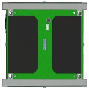
\includegraphics[height=7mm]{cube-icon}}};
}

%digram showing bias windows for the alignment algorithm

\begin{tikzpicture}


    \def\incline{90}                            % Orbit Inclination (degrees)
    \def\poleWindow{10}                         % Polar alignment windows in degrees
    \def\offset{10}                             % Amount the window is offset in the wake direction (i.e.  earlier) in degrees eq_window = 15;
    \def\eqWindow{15}                           % Equatorial alignment window in degrees
    %\def\latTrigger{\incline-\poleWindow}       % Corrects polar window for inclination angle
    \def\latTrigger{80}                         % Corrects polar window for inclination angle

    \def\winR{3cm}                                %window radius for drawing
    \def\axisLen{4cm}

    %import earth background
    \pgftext{
\includegraphics[height=4cm]{earth}}

    %draw orbit
    \draw[->,black,thin] (0,0) circle (\winR);

    %draw axis
    \draw[<->] (-\axisLen,0) -- (\axisLen,0);
    \draw[<->] (0,-\axisLen) -- (0,\axisLen);

    {
        \tikzset{>=triangle 45} %make a bigger arrow
        \draw[->] (25:\winR+0.5cm) arc (25:45:\winR+0.5cm);
        \draw[winLbl]   (35:\winR+0.5cm) node[anchor=south west] {\small Orbit Direction};
    }


    %draw bias windows
    %northbound equatorial window
    \draw[green]                    (0,0)  -- (\eqWindow/2 - \offset:\winR) arc (\eqWindow/2 - \offset:-\eqWindow/2 - \offset:\winR) -- cycle;
    \fill[nearly transparent,green] (0,0)  -- (\eqWindow/2 - \offset:\winR) arc (\eqWindow/2 - \offset:-\eqWindow/2 - \offset:\winR) -- cycle;

    \draw[green,winLbl] (-\offset:\winR+0.5cm) node[anchor=north west] {\small Northbound Equatorial Window};
    \cubesat{-\offset}{\winR}


    %south bound equatorial window
    \draw[red]                    (0,0)  -- (180-\eqWindow/2 - \offset:\winR) arc (180-\eqWindow/2 - \offset:180 +\eqWindow/2 - \offset:\winR) -- cycle;
    \fill[nearly transparent,red] (0,0)  -- (180-\eqWindow/2 - \offset:\winR) arc (180-\eqWindow/2 - \offset:180 +\eqWindow/2 - \offset:\winR) -- cycle;

    \draw[red,winLbl] (180-\offset:\winR+0.5cm) node[anchor=south east] {\small Southbound Equatorial Window};
    \cubesat{180-\offset}{\winR}


    %north polar window
    \draw[blue]                    (0,0)  -- (\latTrigger - \offset:\winR) arc (\latTrigger - \offset:90:\winR) -- cycle;
    \fill[nearly transparent,blue] (0,0)  -- (\latTrigger - \offset:\winR) arc (\latTrigger - \offset:90:\winR) -- cycle;

    \draw[blue,winLbl] (90-\poleWindow/2-\offset/2:\winR+0.5cm) node[anchor=south west] {\small North Polar Window};

    %draw CubeSat
    \cubesat{90-\poleWindow/2-\offset/2}{\winR}

    %draw axis labels
    \draw (0,\axisLen) node[anchor=south] {N};
    \draw (\axisLen,0) node[anchor=west] {E};

    \draw (0,-\axisLen) node[anchor=north] {S};
    \draw (-\axisLen,0) node[anchor=east] {W};

\end{tikzpicture}

    \caption{Bias windows for alignment mode}
    \label{fig:windows}
\end{figure}

As \autoref{fig:windows} the bias windows are offset so that they occur just before the equator or pole. The reason for this is shown in \autoref{fig:winplace}.

\begin{figure}[H]
    \centering
    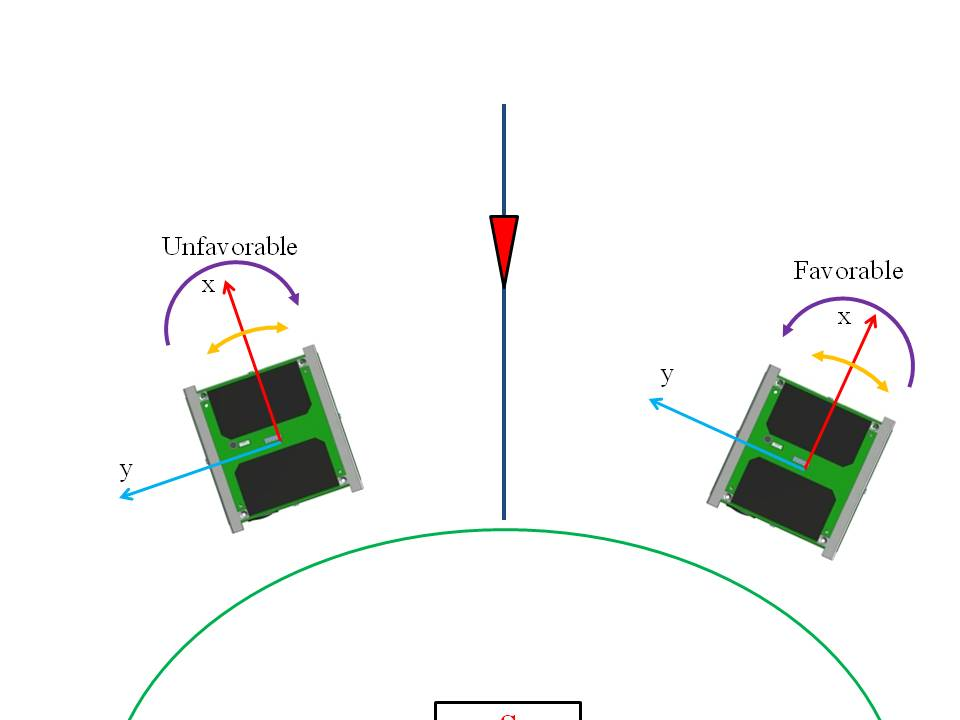
\includegraphics[width=0.5\textwidth]{Windows}
    %\caption{Bias window offset\protect\cite{Mentch11}}
    \caption{Bias window offset}
    \todo[inline]{Figure taken from Crank}
    \label{fig:winplace}
\end{figure}


\subsection{Mode 2}

Mode 2 is initiated at the end of the detumble phase. In mode 2 the torquers are biased as shown in \autoref{fig:m2b} and while the bias is active the algorithm in \autoref{eqn:crossl} is used to dampen out the oscillations caused by the bias. Outside the three bias windows all torquers are set to cancel each other and the \ac{ARC} coasts.

\begin{figure}[H]
    \centering
    %NOTE: this was lifted from Crank
    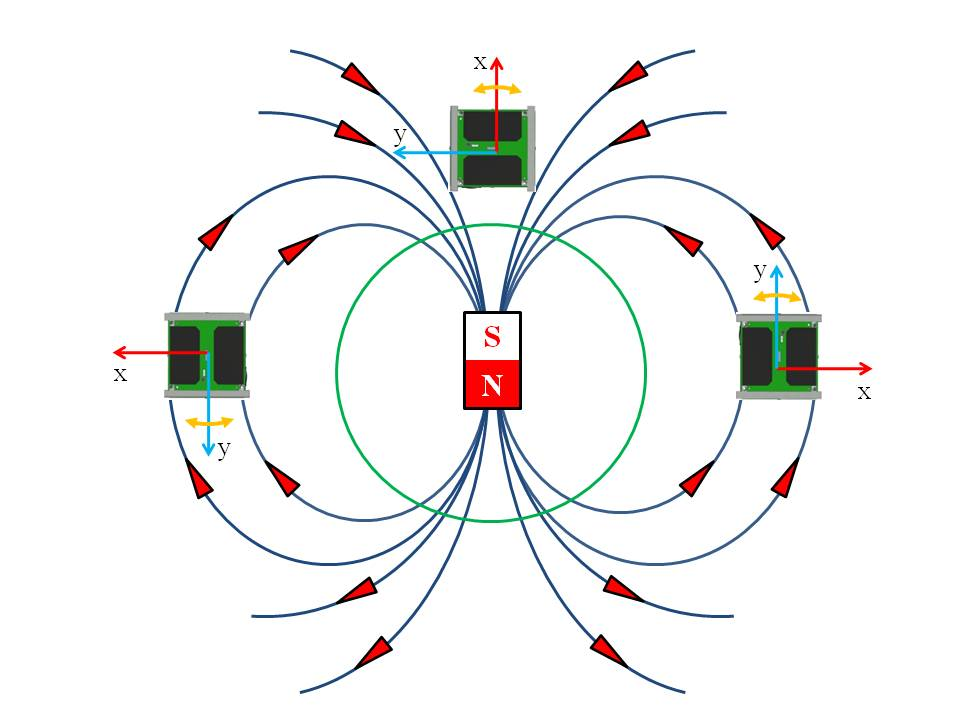
\includegraphics[width=0.5\textwidth]{Figures/Mode-2-Bias}
    %\caption{Bias regions for mode 2\protect\cite{Mentch11}}
    \caption{Bias regions for mode 2}
    \todo[inline]{Figure taken from Crank}
    \label{fig:m2b}
\end{figure}

\subsection{Mode 3}

Mode 3 is initiated after mode 2 is complete. In mode 3 only the north pole bias window is used as shown in \autoref{fig:m3b}. Outside the bias window however the algorithm in \autoref{eqn:crossl} is used to maintain attitude.

\begin{figure}[H]
    \centering
    %NOTE: this was lifted from Crank
    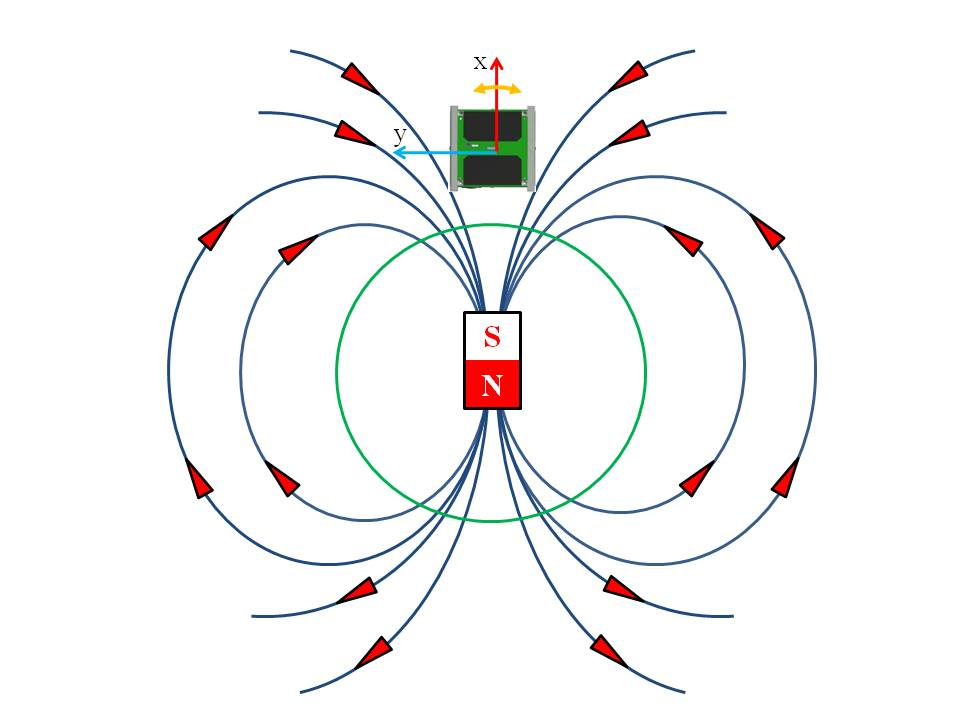
\includegraphics[width=0.5\textwidth]{Figures/Mode-3-Bias}
    %\caption{Bias region for mode 3\protect\cite{Mentch11}}
    \caption{Bias region for mode 3}
    \todo[inline]{Figure taken from Crank}
    \label{fig:m3b}
\end{figure}

\section{Concept of Operations}

%\subsection{Orbital Insertion}

%\ac{ARC} will be ejected from the \ac{PPOD} into orbit. Because CubeSat regulations it will not be posible for \ac{ARC} to have a clock running which could be used to calculate where \ac{ARC} is. Additionally the orbit for \ac{ARC} could change after it has been loaded onto the launch vehicle. For this reason it is not possible for the \ac{ARC} to compute its position without ground station uplink. It is also not within the scope of this thesis to determine the orbit using magnetic field data although it may be possible. Good knowledge of \acs{ARC} location is necessary to calculate the geomagnetic field for use by the Kalman filter. 

%\subsection{Kalman filter lockup}

%The Kalman filter will take some time to converge to a solution. During this time the state estimates of the filter should not be used for attitude control. Because \ac{ARC} will initially have no idea where it is the geomagnetic field will not be known. To allow for filter lockup a static field will be assumed \todo{figure out what field to chose}. This will cause some error in the calculated rotation rates but this should be acceptable for the beginning part of the detumble phase.

\subsection{detumble}

The goal of the detumble mode is to reduce the rotation rates down to an acceptable level \todo{possibly call out such a level}.

%\subsubsection{upload orbital information}

%To correctly calculate attitude and rotation rates orbital parameters must be uplinked. Before this happens detumble can not complete. Once the orbital parameters are uplinked the Kalman filter will likely have to re-adjust which may necessitate that detumble stop for a short period. Once the filter has re-adjusted detumble will still likely have to run for a bit to get the rates within tolerances.

\subsection{alignment}

Once detumble is complete the alignment procedure begins. The alignment procedure takes a fixed 12 \todo{Double check this number} orbits to complete.

\subsubsection{Attitude Determination}

The original design did not use attitude determination to get the satellite into the proper orientation. Instead the rotation rates are used along with the bias windows to get the satellite into the right alignment. The problem is that computing the rotation to the needed accuracy is not a simple process. The original idea was that the rotation rates could be computed directly from magnetic field measurements. A set of magnetometer measurements would be taken each time step to compute the rotation rates. The problem is that to do the rotation rate calculation a derivative is needed. Numerical differentiation is possible but it tends to increase noise by acting as a high pass filter.

The proposed rate determination algorithm also falls short because it does not estimate the full rotation rates. Because the magnetic field is used to determine rotation rates rotations around the magnetic field can not be resolved. This was thought not to be an issue because these rotations are also the kind that can not be corrected for by the torquers but it was shown,in simulation, that removing the component of the rotation rates parallel to the magnetic field caused the CubeSat not to stabilize into the proper alignment. 

To solve both of these problems a Kalman filter is used to estimate both the attitude and the rotation rates using the magnetic field data. The Kalman filter estimates the rates by using the assumed satellite dynamics along with a magnetic field model. The Kalman filter uses the knowledge of the system dynamics to smooth the rate estimates and reduce noise. 



\begin{comment}

\begin{equation}
    F_k = 
        \begin{bmatrix}
              0                &   \hat {\omega} _3 & - \hat {\omega} _2  & \frac{1}{2} & 0           & 0           \\
            - \hat {\omega} _3 &   0                &   \hat {\omega} _1  & 0           & \frac{1}{2} & 0           \\
              \hat {\omega} _2 & - \hat {\omega} _1 &   0                 & 0           & 0           & \frac{1}{2} \\
            0 & 0 & 0 & 0                  & K_1 \hat{\omega}_3 & K_1 \hat{\omega}_2 \\
            0 & 0 & 0 & K_2 \hat{\omega}_3 & 0                  & K_2 \hat{\omega}_1 \\
            0 & 0 & 0 & K_3 \hat{\omega}_2 & K_3 \hat{\omega}_1 & 0                  \\
        \end{bmatrix}
\end{equation}

\begin{equation}
    \Phi \left( t \right) = \matt{I} + \matt{F} t = 
        \begin{bmatrix}
              1                  &   \hat {\omega} _3 t & - \hat {\omega} _2 t  & \frac{1}{2} t & 0             & 0             \\
            - \hat {\omega} _3 t &   1                  &   \hat {\omega} _1 t  & 0             & \frac{1}{2} t & 0             \\
              \hat {\omega} _2 t & - \hat {\omega} _1 t &   1                   & 0             & 0             & \frac{1}{2} t \\
            0 & 0 & 0 & 1                    & K_1 \hat{\omega}_3 t & K_1 \hat{\omega}_2 t \\
            0 & 0 & 0 & K_2 \hat{\omega}_3 t & 1                    & K_2 \hat{\omega}_1 t \\
            0 & 0 & 0 & K_3 \hat{\omega}_2 t & K_3 \hat{\omega}_1 t & 1                    \\
        \end{bmatrix}
\end{equation}

\begin{equation}
    \matt{Q} = Q \matt{I}
\end{equation}

\begin{equation}
    \matt{Q}_k = \int _0 ^ {T_s} \matt{\Phi} \left( \tau \right) \matt{Q} \matt{\Phi} \transpose \left( \tau \right) d\tau = Q \int _0 ^ {T_s} \matt{\Phi} \left( \tau \right) \matt{\Phi} \transpose \left( \tau \right) d\tau
\end{equation}


\begin{equation}
    \matt{Q}_k = Q \int _0 ^ {T_s} \matt{\Phi} \left( \tau \right) \matt{\Phi} \transpose \left( \tau \right) d\tau
\end{equation}

\end{comment}

\subsection{operations mode}

Once alignment is complete the \ac{ACDS} transitions into operations mode. In operations mode the \ac{ACDS} maintains alignment with the desired attitude.

\subsubsection{detect/correct alternate stable configurations}

In operations mode the \ac{ACDS} will check to see if \ac{ARC} has settled into an alternate stable configurations and correct for such conditions. If a correction is made the \ac{ACDS} drops back to alignment mode after the correction is complete.

\subsection{Contingency}

Because the \ac{ACDS} is an experimental system there is a high likelihood that things will go wrong. To account for this the software is written in a way that allows the operation to be changed in case of poor performance. All the Kalman filter parameters and attitude control parameters will be changeable via ground station command.



